\subsection*{Problema 18}
\textbf{Enunciado:} Evaluar la integral definida 
mediante sumas de Riemann usando una 
partición regular sobre el intervalo $[-2, 2]$:
\begin{align*}
\int_{-2}^{2} (x^2 - 2x + 2) \, dx
\end{align*}

\textbf{Solución:} 
Definimos la función $f(x) = x^2 - 2x + 2$ 
en el intervalo $[a, b] = [-2, 2]$. 
La longitud del intervalo es:
\begin{align*}
b - a = 2 - (-2) = 4
\end{align*}

Usamos una partición regular de $n$ subintervalos 
con ancho $\Delta x$:
\begin{align*}
\Delta x = \dfrac{4}{n}
\end{align*}

Los puntos extremos de los subintervalos 
derechos son $x_i = a + i\Delta x$:
\begin{align*}
x_i = -2 + \dfrac{4i}{n}
\end{align*}

Planteamos la suma de Riemann usando el 
extremo derecho:
\begin{align*}
S_n &= \sum_{i=1}^{n} f(x_i) \Delta x \\
S_n &= \sum_{i=1}^{n} f\left(-2 + \dfrac{4i}{n}\right) \left(\dfrac{4}{n}\right)
\end{align*}

Evaluamos la función en $x_i$:
\begin{align*}
f(x_i) &= \left(-2 + \dfrac{4i}{n}\right)^2 
- 2\left(-2 + \dfrac{4i}{n}\right) + 2 \\
f(x_i) &= 4 - \dfrac{16i}{n} + \dfrac{16i^2}{n^2} 
+ 4 - \dfrac{8i}{n} + 2 \\
f(x_i) &= \dfrac{16i^2}{n^2} - \dfrac{24i}{n} + 10
\end{align*}

Multiplicamos por $\Delta x = \dfrac{4}{n}$:
\begin{align*}
f(x_i)\Delta x &= \left(\dfrac{16i^2}{n^2} 
- \dfrac{24i}{n} + 10\right)\left(\dfrac{4}{n}\right) \\
f(x_i)\Delta x &= \dfrac{64i^2}{n^3} 
- \dfrac{96i}{n^2} + \dfrac{40}{n}
\end{align*}

Aplicamos el operador suma y las 
fórmulas estándar:
\begin{align*}
S_n &= \sum_{i=1}^{n} \left(\dfrac{64i^2}{n^3} 
- \dfrac{96i}{n^2} + \dfrac{40}{n}\right) \\
S_n &= \dfrac{64}{n^3}\sum_{i=1}^{n} i^2 
- \dfrac{96}{n^2}\sum_{i=1}^{n} i 
+ \dfrac{40}{n}\sum_{i=1}^{n} 1
\end{align*}

Sustituimos las fórmulas de suma:
$\sum i = \dfrac{n(n+1)}{2}$ y 
$\sum i^2 = \dfrac{n(n+1)(2n+1)}{6}$:
\begin{align*}
S_n &= \dfrac{64}{n^3}\left[\dfrac{n(n+1)(2n+1)}{6}\right] \\
&\quad - \dfrac{96}{n^2}\left[\dfrac{n(n+1)}{2}\right] 
+ \dfrac{40}{n}(n)
\end{align*}

Simplificamos cada término algebraicamente:
\begin{align*}
S_n &= \dfrac{32(2n^2 + 3n + 1)}{3n^2} 
- \dfrac{48(n + 1)}{n} + 40 \\
S_n &= \left(\dfrac{64}{3} + \dfrac{32}{n} 
+ \dfrac{32}{3n^2}\right) - \left(48 + \dfrac{48}{n}\right) + 40
\end{align*}

Agrupamos los términos constantes y en función de $n$:
\begin{align*}
S_n &= \left(\dfrac{64}{3} - 48 + 40\right) 
+ \left(\dfrac{32}{n} - \dfrac{48}{n}\right) 
+ \dfrac{32}{3n^2} \\
S_n &= \dfrac{40}{3} - \dfrac{16}{n} + \dfrac{32}{3n^2}
\end{align*}

Tomamos el límite cuando $n \to \infty$:
\begin{align*}
\int_{-2}^{2} (x^2 - 2x + 2) \, dx &= \lim_{n \to \infty} S_n \\
&= \lim_{n \to \infty} \left(\dfrac{40}{3} - \dfrac{16}{n} + \dfrac{32}{3n^2}\right) \\
&= \dfrac{40}{3} - 0 + 0 = \dfrac{40}{3}
\end{align*}

El valor exacto de la integral definida es $\dfrac{40}{3}$.

\begin{figure}[H]
	\centering
	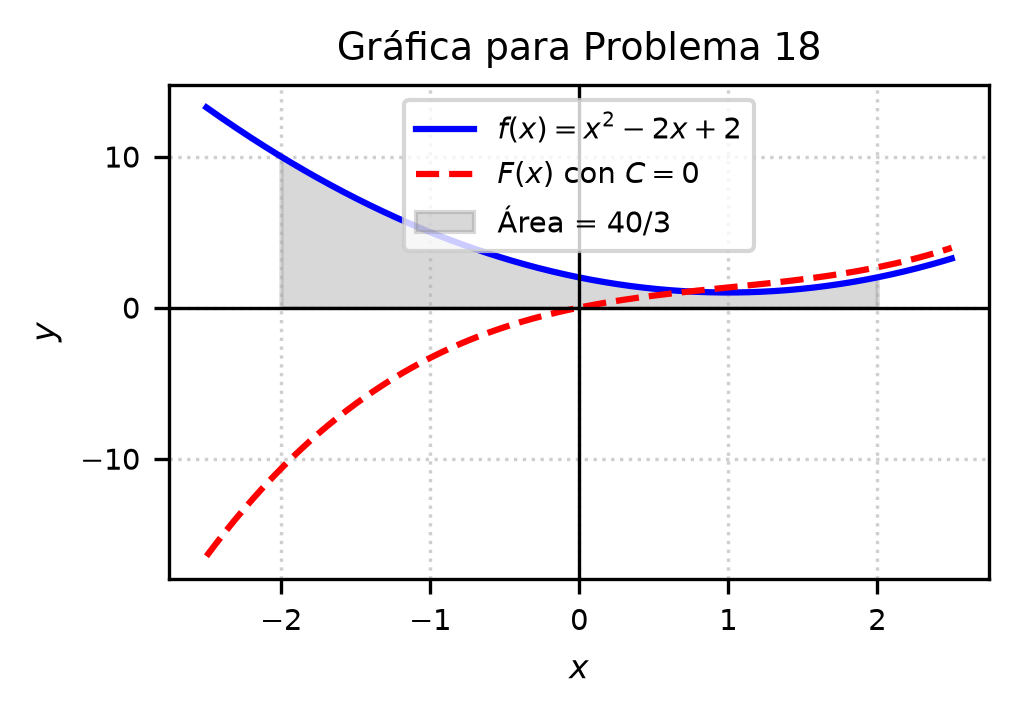
\includegraphics[width=\columnwidth]{semana_06/graficas/SEM06_P18_grafica.png}
	\caption{Representación gráfica de $f(x)$ y su antiderivada $F(x)$ evaluada para la constante de integración $C = 0$ (Problema 18).}
	\label{fig:problema18}
\end{figure}
